\documentclass[8pt, aspectratio=43]{beamer}

\usepackage{HPE_Lecture}
%\usetikzlibrary{arrows.meta} %In HPE_Lecture.sty eingefügt! (Tikz - Bilder in LaTeX)
\usepackage{ifthen} %usepackage um eine if-Verzweigung zu benutzen
\usepackage{tikz}
\usetikzlibrary{angles, calc}

% % % % % % % % % % % % % % % % % % % % % % % % % % %

%Dokument mit allen Ziegerdiagrammen, die im Skript für NuS II enthalten sind. 

% % % % % % % % % % % % % % % % % % % % % % % % % % %

\begin{document}
	
%%%%%%%%%%%%%%%%%%%%%%%%%%%%%%%%%%%%%%%%%%%%%%%%%%%%%%%%%%%%%%%%%%%%%%%%%%%

\begin{frame}\frametitle{Zeigerdiagramm I}

%		\tikzsetnextfilename{Zeigerdiagramm_I_a}
%		\begin{tikzpicture}
%		
%		\end{tikzpicture}

\end{frame}

%%%%%%%%%%%%%%%%%%%%%%%%%%%%%%%%%%%%%%%%%%%%%%%%%%%%%%%%%%%%%%%%%%%%%%%%%%%

\begin{frame}\frametitle{Zeigerdiagramm II}



%		\tikzsetnextfilename{Zeigerdiagramm_RLC_Serie_funter_Schleife}
%		\begin{tikzpicture}
%	
%		\end{tikzpicture}


\end{frame}

%%%%%%%%%%%%%%%%%%%%%%%%%%%%%%%%%%%%%%%%%%%%%%%%%%%%%%%%%%%%%%%%%%%%%%%%%%%

\begin{frame}\frametitle{Zeigerdiagramm III}

	\tikzsetnextfilename{Zeigerdiagramm_III_a_b_c_d}
	\begin{tikzpicture}
		%In der folgenden eckigen Klammer können verschiedene Styles definiert werden,
		%welche dann in diesem tikzpicture verwendet werden können. 
		[Spannungspfeil/.style={-{Latex[length=2mm]},thick, blue},	%Definiert den Style der Sannungspfeile
		 Strompfeil/.style={-{Latex[length=2mm]},thick, red},		%Definiert den Sytle der Strompfeile
		 Winkelpfeil/.style={pic text=$\varphi$, draw, -{Latex[length=1mm]}, angle radius = 7mm, angle eccentricity=1.2},										   %Sytle der  Winkelpfeile
		 Winkelpfeil2/.style={pic text=$\varphi$, draw, -{Latex[length=1mm]}, angle radius = 4mm, angle eccentricity=1.4},										   %Style des kleineren Winkelpfeils von Diagramm d) 
		 Beschriftung/.style={anchor=north, gray}					%Style der Diagrammbeschriftungen a), b), ...
		]
		
		%% Definitionen wie Zeigerlänge und Abstand der Grafiken %%  
		\def\USpitze{1.5cm};	%Länge des Spannungspfiles
		\def\ISpitze{1cm};		%Länge des Strompfeiles
		\def\Winkel{35};		%Winkel zwischen Strom und Spannung
		\def\Xstep{0.3cm};		%Horizontaler Abstand der Grafiken
		\def\BeschSpace{0.25cm};%Vertikalen Abstand der Beschriftung zum waagerechten Pfeil. 
		% ---------------------------------------------------------------------- % 
		%% Diagramm a) %%
		% Koordinaten a) %
		\coordinate (Aa) at (-\Winkel:\ISpitze);	%Koordinaten Definition in Polarform (Winkel:Länge)
		\coordinate (Ba) at (0:0cm);				% Ax ist Spitze des Strompfeils, Bx ist Beginn des Strompfeils
		\coordinate (Ca) at (0:\USpitze);			%Cx ist Spitz des Spannungspfeiles
		% Pfeile a) % 
		\draw[Spannungspfeil] (Ba) -- (Ca) node[midway, above] {$\mzeiger{u}$}; %Spannungspfeil von Bx nach Cx, inkl. Beschriftung
		\draw[Strompfeil] (Ba) -- (Aa) node[midway, below] {$\mzeiger{i}$};		%Strompfeil von Bx nach Ax, inkl. Beschriftung
		\path (Aa) -- (Ba) -- (Ca) pic[Winkelpfeil] {angle = Aa--Ba--Ca};		%Zeichnet den Winkel ein mit Hilfe von pic
		% Beschriftung a) %
		\node[Beschriftung] at (-90:\BeschSpace) {a)};	%Fügt dem Diagramm Beschriftung a) zu. 
		% ---------------------------------------------------------------------- % 
		%% Diagramm b) %% 
		% Koordinaten b) % 
		\coordinate (Bb) at ($(Ca) + (0:\Xstep)$);			%Dank calc library können Koordinaten berechnet werden. 
		\coordinate (Ab) at ($(Bb) + (0:\ISpitze)$);		%Somit können Koordinaten alle relativ berechnet werden
		\coordinate (Cb) at ($(Bb) + (\Winkel:\USpitze)$);
		% Pfeile b) %
		\draw[Spannungspfeil] (Bb) -- (Cb) node[midway, above] {$\mzeiger{u}$};
		\draw[Strompfeil] (Bb) -- (Ab) node[midway, below] {$\mzeiger{i}$};
		\path (Ab) -- (Bb) -- (Cb) pic[Winkelpfeil] {angle = Ab--Bb--Cb};
		% Beschriftung b) %
		\node[Beschriftung] at ($(Bb) + (-90:\BeschSpace)$) {b)};
		% ---------------------------------------------------------------------- % 
		%% Diagramm c) %%
		% Koordinaten c) %
		\coordinate (Bc) at ($(Ab) + (0:\Xstep)$);
		\coordinate (Ac) at ($(Bc) + (0:\ISpitze)$);
		\coordinate (Cc) at ($(Ac) + (180+\Winkel:\USpitze)$); %Cc ist hier der Beginn des Spannungspfeiles
		% Pfeile c) %
		\draw[Spannungspfeil] (Cc) -- (Ac) node[midway, below] {$\mzeiger{u}$};
		\draw[Strompfeil] (Bc) -- (Ac) node[midway, above] {$\mzeiger{i}$};
		\path (Bc) -- (Ac) -- (Cc) pic[Winkelpfeil] {angle = Bc--Ac--Cc};
		% Beschriftung c) %
		\node[Beschriftung] at ($(Bc) + (-90:\BeschSpace)$) {c)};
		% ---------------------------------------------------------------------- % 
		%% Diagramm d) %%
		% Koordinaten d) %
		\coordinate (Bd) at (-90:\ISpitze);
		\coordinate (Ad) at ($(Bd) + (-\Winkel:{\ISpitze/sqrt(2)})$);
		\coordinate (Cd) at ($(Bd) + (0:{\USpitze/sqrt(2)})$);
		% Pfeile d) %
		\draw[Spannungspfeil] (Bd) -- (Cd) node[near end, above] {$\underline{U}$};
		\draw[Strompfeil] (Bd) -- (Ad) node[midway, below] {$\underline{I}$};
		\path (Ad) -- (Bd) -- (Cd) pic[Winkelpfeil2] {angle = Ad--Bd--Cd};
		% Beschriftung d) %
		\node[Beschriftung] at ($(Bd) + (-90:\BeschSpace)$) {d)};
		% ---------------------------------------------------------------------- % 
				
	\end{tikzpicture}
	
	\tikzsetnextfilename{Zeigerdiagramm_III_e}
	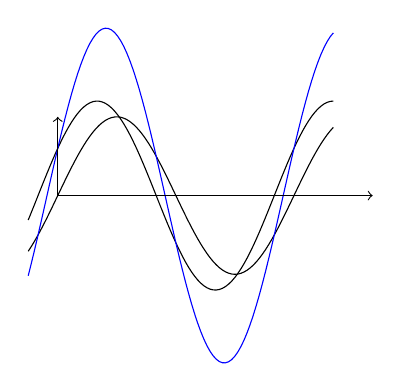
\begin{tikzpicture}
	[domain=-45:420,samples=100,variable=\t]
	
	%\draw[domain=0:6.28,samples=100] plot (\x,{sin(2*\x r)}) node[right] {$f(x) = \sin x$};
	%\draw[scale=0.5,domain=-3.141:3.141,smooth,variable=\t] plot ({\t*sin(\t r)},{\t*cos(\t r)});
	\draw plot (\t/120,{sin(\t)});
	\draw plot (\t/120,{1.2*sin(\t+30)});
	\draw[color=blue] plot (\t/120,{sin(\t)+1.2*sin(\t+30)});

	\draw[->] (0:0) -- (90:1cm);
	\draw[->] (0:0) -- (0:4cm);

	
	\end{tikzpicture}
	
	
\end{frame}

%%%%%%%%%%%%%%%%%%%%%%%%%%%%%%%%%%%%%%%%%%%%%%%%%%%%%%%%%%%%%%%%%%%%%%%%%%%%%

\end{document}

